% @Author: Taha Bouhsine


%%%%%%%%%%%%%%%%%%%%%%%%%%%%
% CHAPTER                  %
%%%%%%%%%%%%%%%%%%%%%%%%%%%%
\setcounter{mtc}{8}
\chapter{Project General Context }%
\label{chap:chapter_one}
\minitoc
%%%%%%%%%%%%%%%%%%%%%%%%%%%%
% SECTION                  %
%%%%%%%%%%%%%%%%%%%%%%%%%%%%
\section{ Project Presentation }
\subsection{Presentation}
Multiple projects and ideas all over the world go to waste and get canceled due to either lack or insufficient funds.
This means the loss of a huge amount of new business chances and opportunities that would have been of great benefit for both individuals and communities.

The result is an extreme demand and concern to come up with a crowdfunding platform the necessary tools for the public to create, fund, and support causes and creative minds all over the world.



\subsection{Problem}
% "Ideas are cheap, Execution is expensive" Even if you create a beautiful application with a beautiful User Interface, if you neglect even one aspect of the main functionalities, and built it with a half effort, you might result in a product that won't live for long, or if you were to use the wrong technologies for the project, you might as well find yourself limited and won't be able to create and bring the most out of your Idea.

For the last few years, all over the world crowdfunding become one of the main tools and funding source for most of the new startups and creative minds all over the globe,
so we sought to create a new crowdfunding application, that will bring and adopt all the creative minds and ambitious souls and provides them with a tool to seek funds from a global community,
the creators should be able to coordinate multiple campaigns easier, and should be able to find people who are willing to invest with little equity involved. And help in gatekeeping that will monitor and create symbiotic relations with other algorithms and information online by using cloud-based solutions for better access.
Our platform can help leap the hurdle of lack of experience in each field. Letting the barrier of entry be lessened for everyone who has a dream.

So for our project, there is a real challenge in creating a product that competes with all the other platforms out there, so we have to try and understand the human's motivation and behavior, what does urge him to help others, or seek the help of others,
a lot of articles helped us along the way, studying the psychological side of human nature and the act of giving, and which factors that affect his decision to give.

\subsection{Main Actors}
Different players are involved in crowdfunding models. First, there are creators, innovators, and entrepreneurs that have ideas and
projects to be funded. They want to use crowdfunding to gather financial support from interested supporters.
Then there is the crowd of people that provides this financial support to these projects, bearing an investment
risk and expecting a certain payoff. And finally, there is the crowdfunding platform, the intermediary that acts
as a matchmaker between those who want to deliver the new initiatives using crowdfunding mechanisms
and those who want to support such initiatives through their investment efforts \cite{crwdfun:transform}.
\begin{enumerate}
      \item Creator:
            Or capital seekers, are mainly concerned with their motivations to get involved in crowdfunding, the determinants of success, and the legal restrictions of equity-based crowdfunding \cite{10.1007/978-3-319-18017-5_3}.

      \item Funder:
      Or capital providers, are essential to the success of a crowdfunding campaign. Interesting research can be performed on the motives of this unique group of investors for participating in crowdfunding. One thing that
            makes this group so special is that they are not exclusively motivated by earning money.

\end{enumerate}
% Creators
\subsubsection*{Creators}
The reasons for people to fund their projects via crowdfunding are wider than just money. Gerber et al. \cite{inproceedings} 
have, by interviewing people involved in crowdfunding, identified the following motivations:
\begin{enumerate}
      \item Raise Funds: 
            Almost trivial, one of the motivations is to raise funds. Also, platforms provide a way to
            collect payments online, and accept small payments from a large number of people. Therefore, capital
            seekers do not need to develop an infrastructure for it.

      \item Establish Relationships and form Connections:        
            In addition to raising funds, one other advantage is the opportunity for a direct connection between creators and funders potentially extending beyond the campaign itself. The
            long term relationship stands in contrast to the short term relationship that occurs in many alternatives
            to crowdfunding.

      \item Maintain Control.

      \item Learn New Fundraising Skills.

      \item Receive Validation and approval:           
            Successful experiences and receiving public recognition of their success increase
            a person’s confidence in his/herself and the project. According to the writers, this finding is consistent
            with social cognitive theory, which suggests that people build beliefs in their ability through social interactions. This finding is supported by prior research in online communities, which finds that people
            engage in these communities to build self-esteem.

      \item Replicate Successful Experience of Others:          
            According to the researchers, initial findings suggest that
            people participate in crowdfunding because they want to replicate the success of others. Creators that
            succeed in funding a project online provide social proof that motivates others to become creators as
            well.

      \item Expands Awareness  of Work  through Social Media:     
            Findings suggest that creators were motivated to
            participate in crowdfunding because it expanded their awareness through social media. In one of the
            interviews in the research, an anthropologist who used the crowdfunding platform RocketHub to fund
            her research on ancient Roman skeletons, described being motivated to not only share her work publicly but engage in a dialogue about her work. She gained a lot of followers on Twitter and has even
            started a blog as a result of her newfound fame.

\end{enumerate}

Creators deterrents to Crowdfunding:
\begin{enumerate}
      \item Inability to Attract Supporters
      \item Fear of Public Failure and Exposure
      \item Time and Resource Commitment
\end{enumerate}

\paragraph*{Factors For Successful Crowdfunding}
\begin{enumerate}
      \item Orientation of the project:     
            Whether the project or the organization behind it is a non-profit or not
            seems to influence the success of funding. Belleflamme et al. \cite{doi:10.1080/13691066.2013.785151} performed an empirical analysis
            to investigate this. They found that non-profit organizations tend to attract larger amounts of money.
            According to them, this finding is in line with earlier research stating that non-profit organizations
            are better at attracting outside funds because of their stronger focus on the social outcome than on
            monetary gains.

      \item Amount and duration:     
            According to that same research \cite{doi:10.1080/13691066.2013.785151}, increasing goal size is negatively associated
            with success. Less expected was that an increased duration of a campaign decreases the chances of
            success. This might be explained as that longer durations are a sign of lack of confidence.

      \item Social network:     
            Research by Agrawal et al. \cite{NBERw16820} indicates the important role that friends and family may
            play in generating early investment in entrepreneurial ventures. They speculate that this early investment may serve as a signal of entrepreneurial commitment. Later investors may use this signal thereby
            increasing the likelihood of further funding by way of access to distant sources of capital.
\end{enumerate}


% Funders
\subsubsection*{Funders}
Funders are essential to the success of a crowdfunding campaign. Interesting research can be performed on the motives of this unique group of investors for participating in crowdfunding. One thing that
makes this group so special is that they are not exclusively motivated by earning money.
In crowdfunding, consumers have taken on the role of investors or capital providers. And they are diverse. Even on the same platform, the motives to make investments can greatly vary between consumers.
Based on earlier research, Lin et al. \cite{doi:10.5465/ambpp.2014.209} have identified a set of motivations that may drive a person’s participation in crowdfunding:

\begin{enumerate}
      \item Seek Rewards:
            At reward-based platforms, capital seekers can offer rewards linked to the size of the contribution by the investor. These rewards range from t-shirts and
            acknowledgment on the project page to pre-ordering the actual product. The latter sometimes leads
            to confusion situations for consumers. Although explicitly disclaimed by Kickstarter, many consumers
            are under the impression that the web site is essentially an online retail storefront in which project
            creators are pre-selling products \cite{10.2139/ssrn.2234765}.

      \item Help Others and support Creators and causes: One of the interviewees from a study carried out by Gerner et al. \cite{inproceedings}
            stated that he funds an idea that he thinks is neat, but he also really likes the idea of people being
            able to get off the ground without needing to buy into a big giant corporate structure.

      \item Engage and Contribute to a Trusting and Creative Community:
            People generally feel like they are involved or engaged in the project
            throughout the duration. Crowdfunding allows a lot of people to be involved in something that
            they maybe otherwise would not have the opportunity to be involved in. Just to be a part of something
            is what motivates people in those cases \cite{inproceedings}.

      \item Reputation:
            Another motivation for many participants of online and crowdsourcing communities is
            the reputation benefits and recognition that can be derived from active participation in the community \cite{doi:10.5465/ambpp.2014.209}.
            Fellow investors on Kickstarter can see what projects you backed. This creates a sense of ’high-profile
            community members’.
\end{enumerate}


One motivation of supporters in crowdfund-ing communities is the desire to collect external rewards such as an acknowledgment, a tangible artifact, or an experience. An acknowledgment may come in the form of a telephone call, while a tangible artifact could be a CD or gadget. An experience may involve, for instance, meeting with the creator. The creator’s goal is to provide rewards that satisfy the supporters’ desire to collect.

\subsection{Design Principles}
Based on these motivations, Gerber et al. \cite{crowdMotiv} developed three design principles for crowdfunding
intermediaries. These principles enhance motivation for these actors to individually decide to become and
stay involved in crowdfunding.

\subsubsection*{Support Resource Export}
Crowdfunding actors should be able to exchange human, information, and financial resources before, during, and after the crowdfunding campaign. The human resources are persons that can help to fulfill tasks
associated with creative production, such as creation, manufacturing, implementation, marketing, planning,
and fulfilling. Examples of information resources are information and explanations.
Access to informational and human resources has been found to have a direct positive impact on persistence
in ambiguous tasks. With financial resources, we refer to funding. Almost all platforms already provide the
exchange of financial resources, as this is fundamental to crowdfunding. The exchange of the other types are
often overlooked. Adding this to the design could potentially enhance a project’s success.
During the preparation stage, capital seekers are advised to search for example projects, read advice blogs,
seek one-on-one advice, and outsource preparation tasks. However, on many intermediaries, users cannot
see unsuccessful campaigns \cite{10.1145/2531602.2531715}.

\subsubsection*{Support community before, during, and after}
Intermediaries could offer users the possibility to interact or meet up before, during, and after the campaign.
There should be opportunities to meet up with potential capital providers to increase awareness of the upcoming project before the campaign starts. During the campaign, there should be tools and channels available to promote the project. And when the campaign is successful, there should be a way to keep supporters
up-to-date about the execution of the project.
According to earlier research, people are more likely to persist when they publically commit beforehand
and then share small wins with others throughout the effort.
Through the sharing process, they receive positive validation and are more likely to believe they can
accomplish a task, are willing to take on more challenging work, have a greater intrinsic motivation 
to complete a task, persist in the face of challenges, and expend
more effort in the task \cite{crowdMotiv}.
The community around crowdfunding developed tools to support after-campaign work. Intermediaries could offer a matchmaking
service to bring together supply and demand \cite{doi:10.5465/ambpp.2014.209}.
% \subsubsection*{Provide transparency}
% On crowdfunding intermediaries, capital seekers pitch their unique ideas to the crowd. The legalities involved
% should be included in the sign-up process. It is important that this is done in a way that is understandable for
% non-experts. Providing a 20-page-long document with all the rules in a language only lawyers can understand
% is not suggested. The same goes for the legalities involved when intermediaries are collecting data on their
% users. Research in psychology and human-computer interaction suggests that transparency creates trust,
% and trust supports future participation.

\subsection{Objectives}

So one of our main objectives is to create a platform that can improve our user's experience and boost the chance of our creators to reach the maximum of the audience as well as facilitate the access and the funding process for our funders, and provide a place where they can build there trust and look for promising talents and empowering entrepreneurs to help in creating new possibilities.

Firstly, we need to make sure
that the code is maintainable for future alterations and additions by other programmers. For this, we will try
to keep the files organized in a logical setup and we will comment our code where necessary, to understand
its workings.

Secondly, « Sahem » platform will deal with sensitive data on several occasions. First of all, there
is the user data, which includes personal information and passwords. Secondly, there is a payment system
that involves sensitive financial information of the users. This is why it is very important to build our system
to be as secure as possible.

Thirdly, the platform needs to have an attractive and clean design. It needs to be user-friendly, easily navigable, and look professional so that users will trust the platform is capable of performing
well in the financial setting. So I came up with a unique design, and tried to create a new experience for the users, fast,
smooth, mobile responsive, and easy interface to interact with.
\begin{enumerate}
      \item
            User Experience:
            Making sure that our crowdfunding software solutions are easy to navigate for the end-user is a crucial part of the development process. If our customers are befuddled by how to navigate our application, then it is highly likely that they will leave and find another crowdfunding platform. Not only will we want a functional interface, but one that is eye-catching as well.
            One thing to take note of is the importance of giving them the terms and conditions within the first few steps, so they fully understand what to expect. This shows a dedication to transparency that many startups and entrepreneurs will appreciate.

      \item
            Account Management:
            Our customers will want to know what is going on, and making it easy on them will help make our platform successful. That means setting up systems that make it very clear what’s going on with their project. We will want them to be able to access who has been investing, how much money they have, how far they are from their goal, and any other metric they need to run a successful campaign. This could also include reports for recharges, withdrawals all available via a simple to navigate dashboard.
      \item
            Report Generation:
            As the platform owner, you need a way to benefit from your time spent on creating this site that will help so many people. So, ensuring you also have access to backed reports like rewards, investors, and such can help you help them, as they say. This means creating a dashboard that, just like for the actual campaign creators, is easy to navigate and gives you access to reports you can use to course-correct and upgrade the systems.
      \item
            Payment Gateway \& Marketing:
            When starting a crowdfunding platform you will want to set it up with access to the right payment gateways. Each gateway has its features, and so doing some in-depth research into them will allow you to choose one or several that works for the largest number of potential customers.
\end{enumerate}



\section{Functionality}
The platforms operate by allowing those seeking finance to make a pitch on the site outlining how much money they need, what they need the money for, if anything, you get in return for contributing. Potential funders can then view pitches on the platform, interact with both those looking for finance and other potential funders, and then decide whether or not they want to back the campaign. The majority of platforms operate the all–or–nothing model where, if the target amount is not raised within a given timeframe, contributions are returned to funders and no financing goes ahead, but we are using the Keep It All model, anything you raise is yours.

When a new user arrives at the landing page he will be greeted with the main interface of the application, that holds multiple pieces of information and presentations of our platform, it explains the basic functionalities and the different advantages of our application.

Our simple design, based on some principles of improving the user's experience found in Krug's book "Don't make me think, revisited: a common sense approach to Web usability", we have chosen to make the most important buttons into unique color from the others, on normal cases the user will click on one of them to navigate to the appropriate page, at first he will have the ability to navigate to the existing fundraiser campaigns of the platform, and if he chooses to fund the project, he will be redirected to the Registration form in order to authenticate, and fill his personal profile, and provide the platform with his credit card information.

After the authentication, he will have the ability to create and submit his own fundraiser.

In his profile, he can see his personal information and get to show all of his achievements, the projects he funded, and the fundraisers he created as well as the posts he published in the platform. 
% TODO 

\section{Feasibility}
This project is technically and financially feasible. I will spend approximately nothing to host the app, and in the future, there is an option to pay as you grow, by generating income from cutting a \% from the funds at the end of each fundraiser, we will get the costs covered. With regards to the technical feasibility, it will be built in well-established MEAN Stack technologies, that have a low cost with great scalability, and maintainability.

« Sahem » provides the following features:
\begin{enumerate}
      \item Trust-building through the corroboration mechanism.
      \item
            Opportunity for long term commitment between Creators and Funders.
      \item
            Uses secure technologies on both the frontend and the backend, and any requests sent by the users are passed by multiple middlewares on the backend.
      \item
            Easy Navigation through simple user interface design built using Angular, a framework that helps in creating fast and reliable Single Page Applications.
      \item
            A headless backend, which allow us to create different frontend application afterward, and that are linked to the same backend.
      \item
            Global crowdfunding interaction, no limits between countries, everyone can fund or create fundraisers.
      % \item
      %       Statistical analysis of need vis-à-vis people.
\end{enumerate}
\section{ Project Management }
Process-driven software development is based on rigorously defined activities and tasks that are also repeatable and measurable. Formal processes facilitate planning, analysis of requirements from multiple angles, design of high-quality software models by following standards and using team-based tools, and incorporation of quality through walkthroughs, inspections, and testing.
As a result, such formal processes enhance quality and maximize user benefits.

\subsection{ Project Development Process }
The process of discipline is complex. This is because a process considers myriad different hard and soft factors that impact development. Many software developers argue that processes restrict their creativity. Far from that, processes enable creativity with value. This is because processes ensure the effort made by architects, designers, developers, and testers will be well directed toward the commonly agreed goals (business objectives) of a project. Processes also facilitate measures and metrics that indicate individual and team productivity and quality. Metrics and measurements in software projects also enable the assignment of responsibilities and accountabilities.
To develop a good product we need a good development method. One very popular agile framework for this is iterations and increments.

The iterations and increments as shown in Figure \ref{fig:iterationlifecycle} are the basis of most modern-day approaches to developing good software. In this iterative and incremental approach, no deliverable is produced in a single attempt. Instead, at least three iterations (repetitions) are undertaken before producing a deliverable.
This is followed by incrementally adding another package, which would have its own three or more iterations. The three terms iteration, incremental, and parallel are further discussed next.
\begin{figure}[!ht]
      \center
      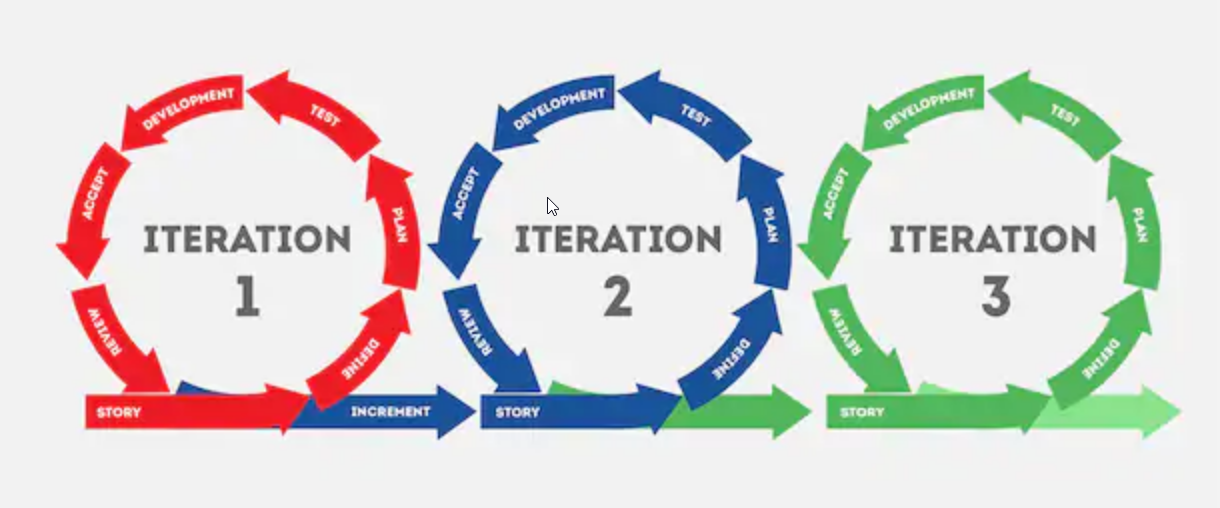
\includegraphics[scale=0.40]{assets/iteration.png}
      \caption{Iterative process project life cycle}
      \label{fig:iterationlifecycle}
\end{figure}

\paragraph*{Iterative}
The iterative aspect of a process enables the repetition of tasks. As a result, the deliverables are produced gradually. For example, when a use case is iterated, additional material is added to the description of the use case—such as alternative flows within the use case. The iterative approach encourages a slow and steady philosophy rather than hurrying and finishing up a deliverable in the first attempt.
Deliverables are gradually matured by undertaking at least three iterations across multiple other deliverables. For example, while following an iterative process one might move from an initial use case to another use case in another diagram, then identify classes and draw a sequence diagram before coming back to the original use case and completing it.

\paragraph*{Incremental}
The incremental aspect of a process enables adding new elements and diagrams to an existing deliverable. An example is to add new packages to existing or developing packages. New requirements are thus discovered and modeled incrementally. This incremental aspect of the process enables the creation of parts of a system in as complete a manner as possible before proceeding with the development of additional parts of the system. The incremental aspect of a process often goes hand in hand with the iterative aspect. For example, while a new deliverable is incrementally added (a new use case), an existing deliverable is iteratively augmented during a later iteration (e.g., additional steps added to a use case).

\subsection{Monitoring And Planning}

\subsubsection*{Monitoring}
Breaking down a project into subparts does help a lot in enabling controlled the execution and monitoring of the project, it helps with keeping the project well displayed and well planned to avoid all the mishaps spaghetti code afterward.
Figure \ref{fig:bos} shows how we divided the business objective into subparts. To arrive at acceptable performance criteria of the system, the BO gets further divided into smaller parts or subject areas.
\begin{figure}[!ht]
      \center
      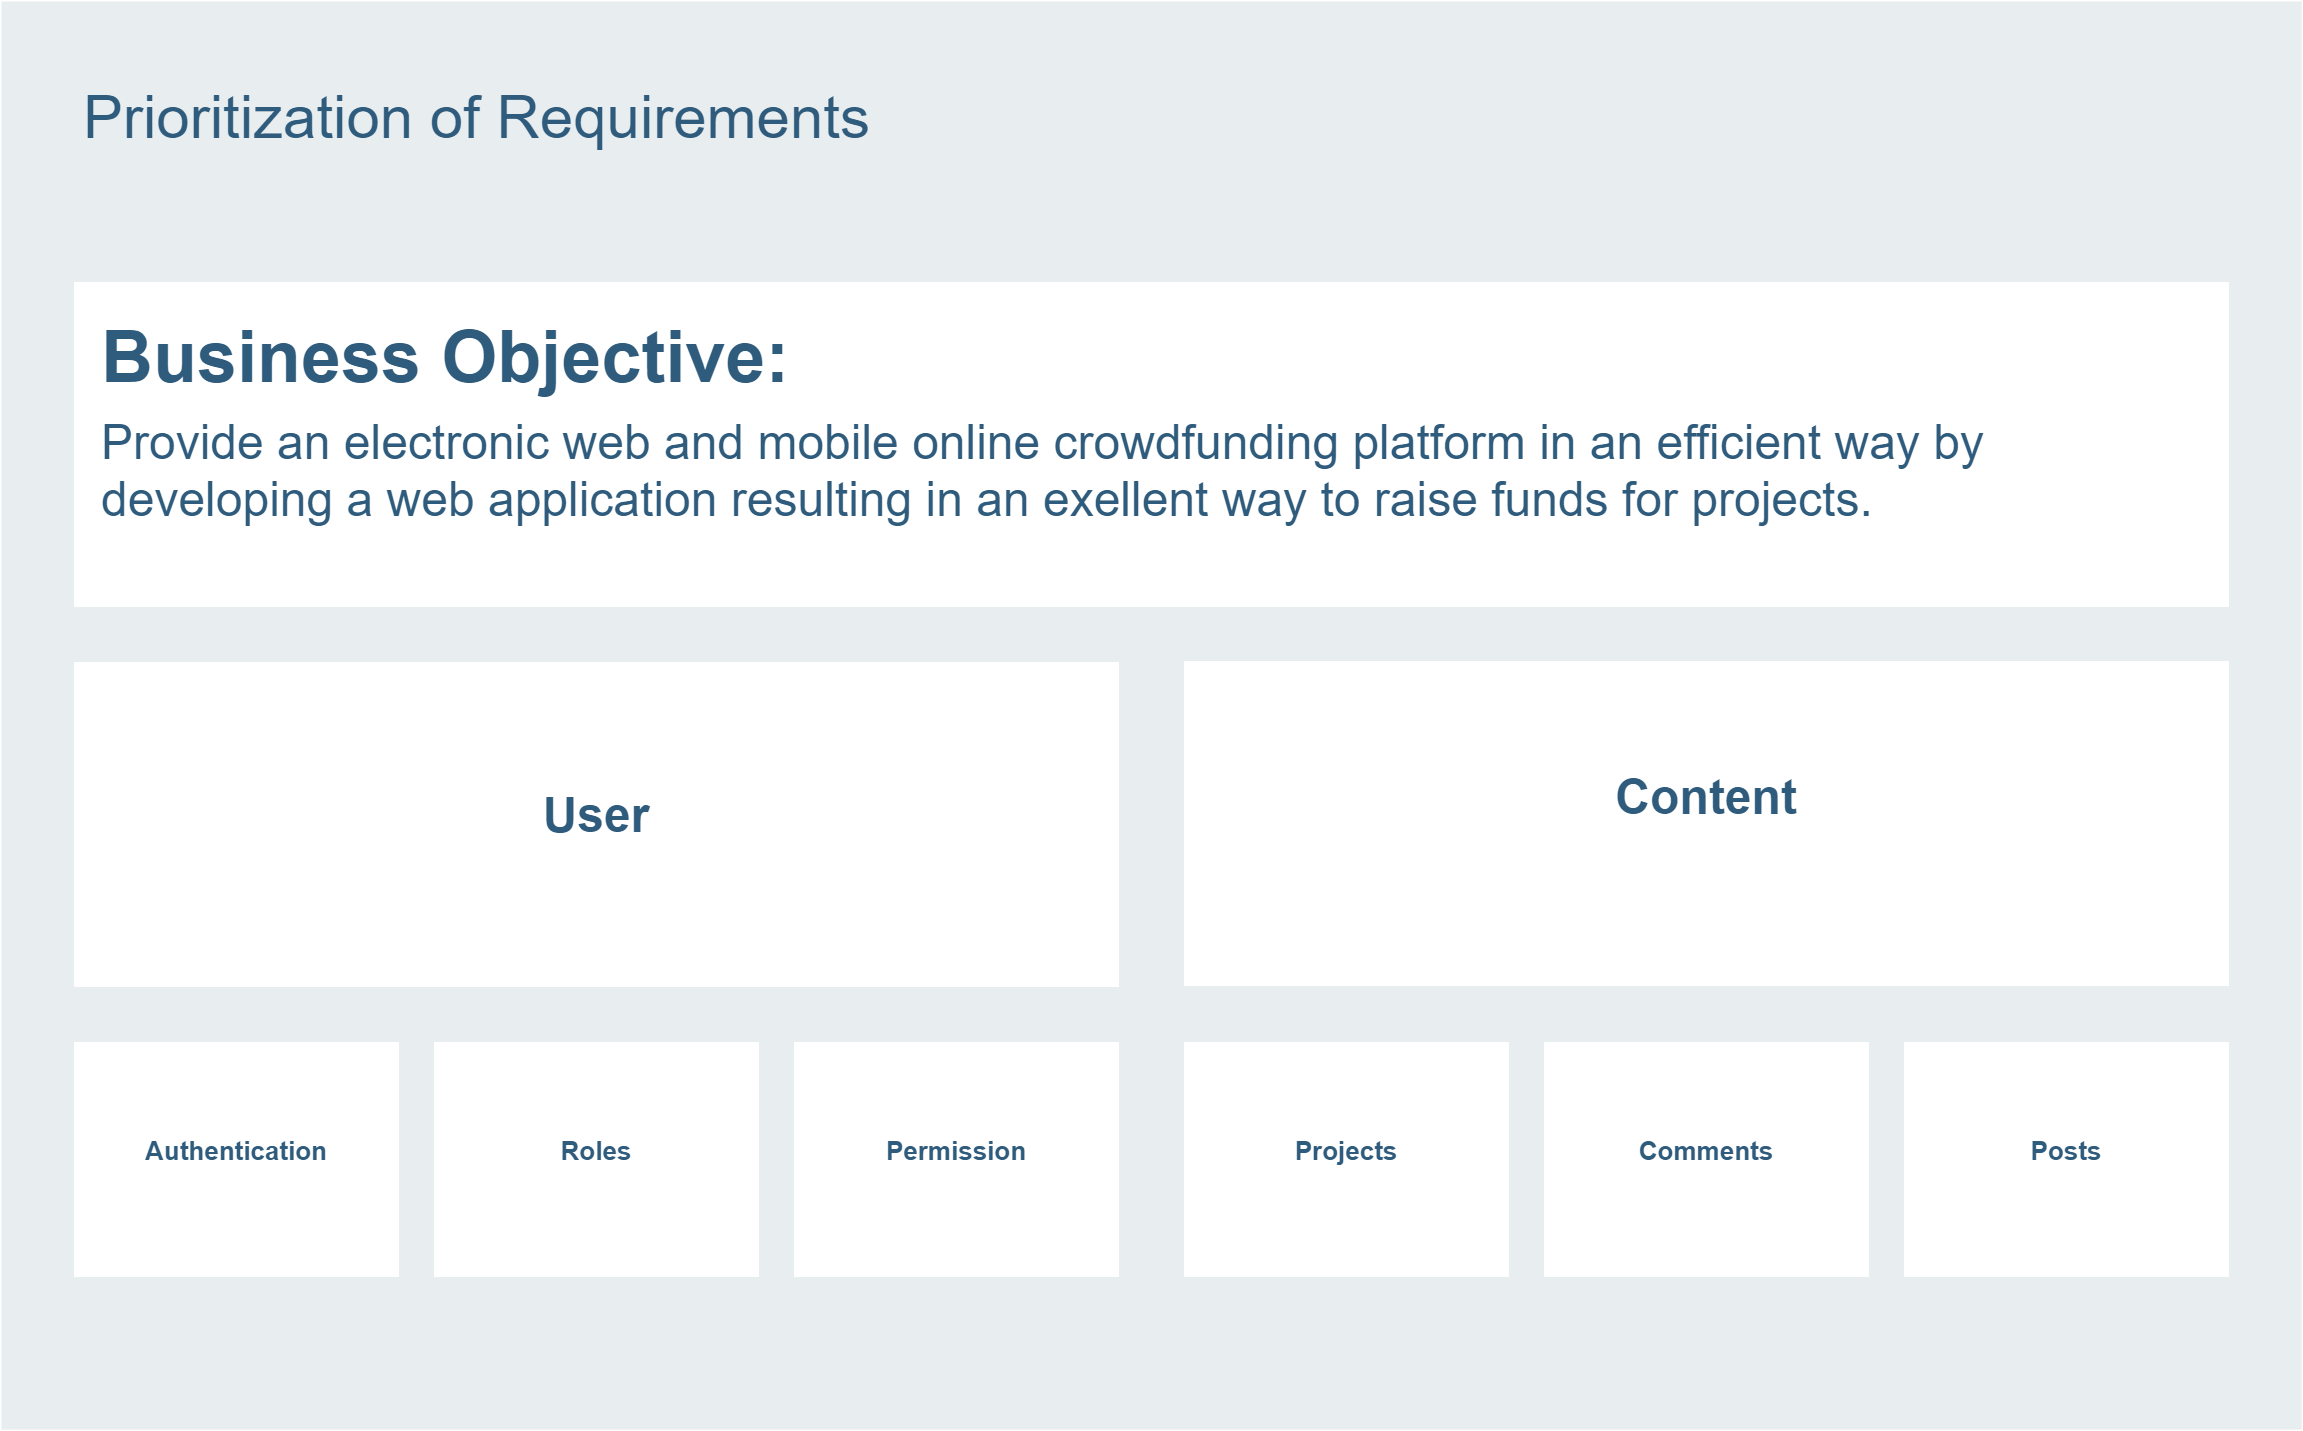
\includegraphics[scale=0.18]{assets/bos.png}
      \caption{« Sahem » Business Objectives}
      \label{fig:bos}
\end{figure}

\subsubsection*{Planning}
During the planning we should provide precise routing of one or more business processes with opportunities to optimize on time and costs associated with the processes.
So we created a Gantt Chart in teamGantt to help us follow the progress of different tasks and the time left to complete them:
% what we did with gantt chart
\clearpage
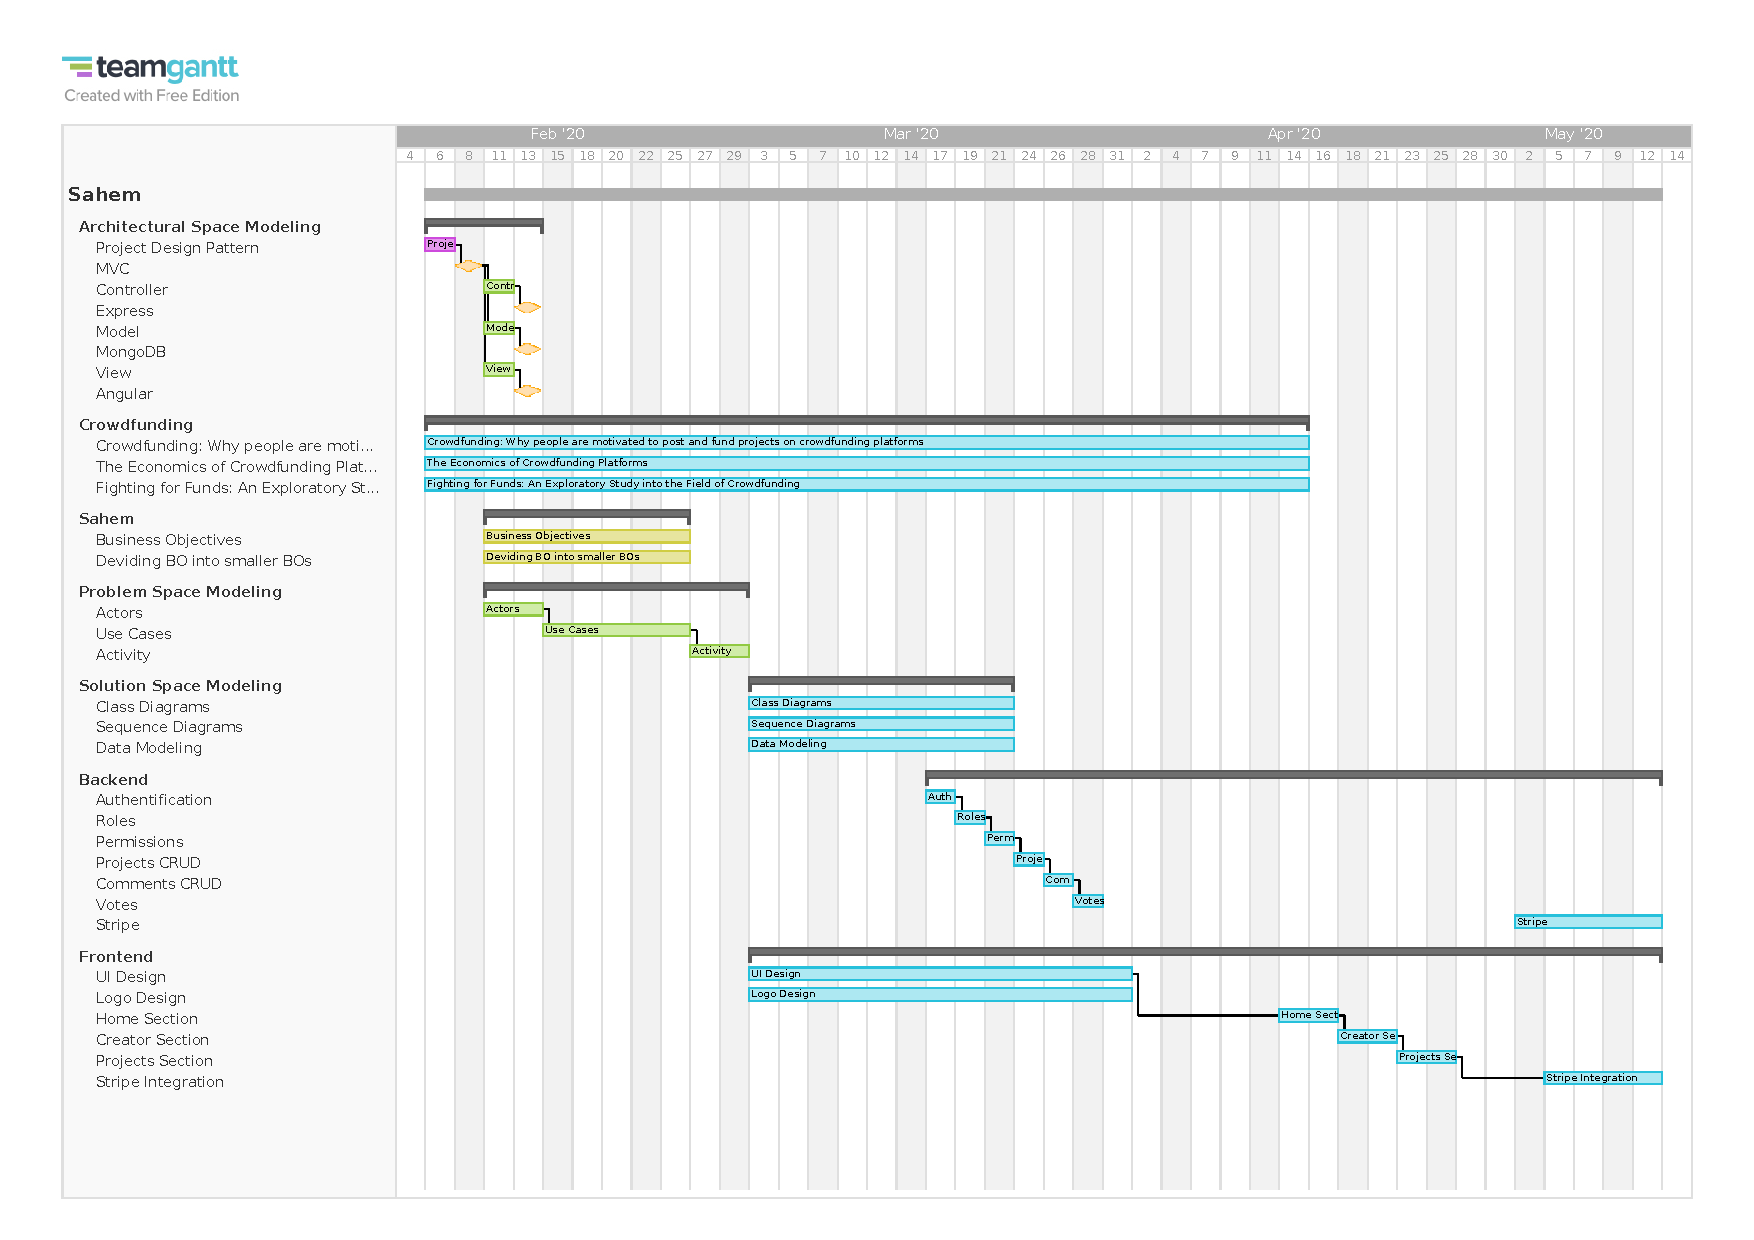
\includepdf[pages=-,angle=90,]{assets/ganttchart.pdf}
